\documentclass[1p]{elsarticle_modified}
%\bibliographystyle{elsarticle-num}

%\usepackage[colorlinks]{hyperref}
%\usepackage{abbrmath_seonhwa} %\Abb, \Ascr, \Acal ,\Abf, \Afrak
\usepackage{amsfonts}
\usepackage{amssymb}
\usepackage{amsmath}
\usepackage{amsthm}
\usepackage{scalefnt}
\usepackage{amsbsy}
\usepackage{kotex}
\usepackage{caption}
\usepackage{subfig}
\usepackage{color}
\usepackage{graphicx}
\usepackage{xcolor} %% white, black, red, green, blue, cyan, magenta, yellow
\usepackage{float}
\usepackage{setspace}
\usepackage{hyperref}

\usepackage{tikz}
\usetikzlibrary{arrows}

\usepackage{multirow}
\usepackage{array} % fixed length table
\usepackage{hhline}

%%%%%%%%%%%%%%%%%%%%%
\makeatletter
\renewcommand*\env@matrix[1][\arraystretch]{%
	\edef\arraystretch{#1}%
	\hskip -\arraycolsep
	\let\@ifnextchar\new@ifnextchar
	\array{*\c@MaxMatrixCols c}}
\makeatother %https://tex.stackexchange.com/questions/14071/how-can-i-increase-the-line-spacing-in-a-matrix
%%%%%%%%%%%%%%%

\usepackage[normalem]{ulem}

\newcommand{\msout}[1]{\ifmmode\text{\sout{\ensuremath{#1}}}\else\sout{#1}\fi}
%SOURCE: \msout is \stkout macro in https://tex.stackexchange.com/questions/20609/strikeout-in-math-mode

\newcommand{\cancel}[1]{
	\ifmmode
	{\color{red}\msout{#1}}
	\else
	{\color{red}\sout{#1}}
	\fi
}

\newcommand{\add}[1]{
	{\color{blue}\uwave{#1}}
}

\newcommand{\replace}[2]{
	\ifmmode
	{\color{red}\msout{#1}}{\color{blue}\uwave{#2}}
	\else
	{\color{red}\sout{#1}}{\color{blue}\uwave{#2}}
	\fi
}

\newcommand{\Sol}{\mathcal{S}} %segment
\newcommand{\D}{D} %diagram
\newcommand{\A}{\mathcal{A}} %arc


%%%%%%%%%%%%%%%%%%%%%%%%%%%%%5 test

\def\sl{\operatorname{\textup{SL}}(2,\Cbb)}
\def\psl{\operatorname{\textup{PSL}}(2,\Cbb)}
\def\quan{\mkern 1mu \triangleright \mkern 1mu}

\theoremstyle{definition}
\newtheorem{thm}{Theorem}[section]
\newtheorem{prop}[thm]{Proposition}
\newtheorem{lem}[thm]{Lemma}
\newtheorem{ques}[thm]{Question}
\newtheorem{cor}[thm]{Corollary}
\newtheorem{defn}[thm]{Definition}
\newtheorem{exam}[thm]{Example}
\newtheorem{rmk}[thm]{Remark}
\newtheorem{alg}[thm]{Algorithm}

\newcommand{\I}{\sqrt{-1}}
\begin{document}

%\begin{frontmatter}
%
%\title{Boundary parabolic representations of knots up to 8 crossings}
%
%%% Group authors per affiliation:
%\author{Yunhi Cho} 
%\address{Department of Mathematics, University of Seoul, Seoul, Korea}
%\ead{yhcho@uos.ac.kr}
%
%
%\author{Seonhwa Kim} %\fnref{s_kim}}
%\address{Center for Geometry and Physics, Institute for Basic Science, Pohang, 37673, Korea}
%\ead{ryeona17@ibs.re.kr}
%
%\author{Hyuk Kim}
%\address{Department of Mathematical Sciences, Seoul National University, Seoul 08826, Korea}
%\ead{hyukkim@snu.ac.kr}
%
%\author{Seokbeom Yoon}
%\address{Department of Mathematical Sciences, Seoul National University, Seoul, 08826,  Korea}
%\ead{sbyoon15@snu.ac.kr}
%
%\begin{abstract}
%We find all boundary parabolic representation of knots up to 8 crossings.
%
%\end{abstract}
%\begin{keyword}
%    \MSC[2010] 57M25 
%\end{keyword}
%
%\end{frontmatter}

%\linenumbers
%\tableofcontents
%
\newcommand\colored[1]{\textcolor{white}{\rule[-0.35ex]{0.8em}{1.4ex}}\kern-0.8em\color{red} #1}%
%\newcommand\colored[1]{\textcolor{white}{ #1}\kern-2.17ex	\textcolor{white}{ #1}\kern-1.81ex	\textcolor{white}{ #1}\kern-2.15ex\color{red}#1	}

{\Large $\underline{12n_{0073}~(K12n_{0073})}$}

\setlength{\tabcolsep}{10pt}
\renewcommand{\arraystretch}{1.6}
\vspace{1cm}\begin{tabular}{m{100pt}>{\centering\arraybackslash}m{274pt}}
\multirow{5}{120pt}{
	\centering
	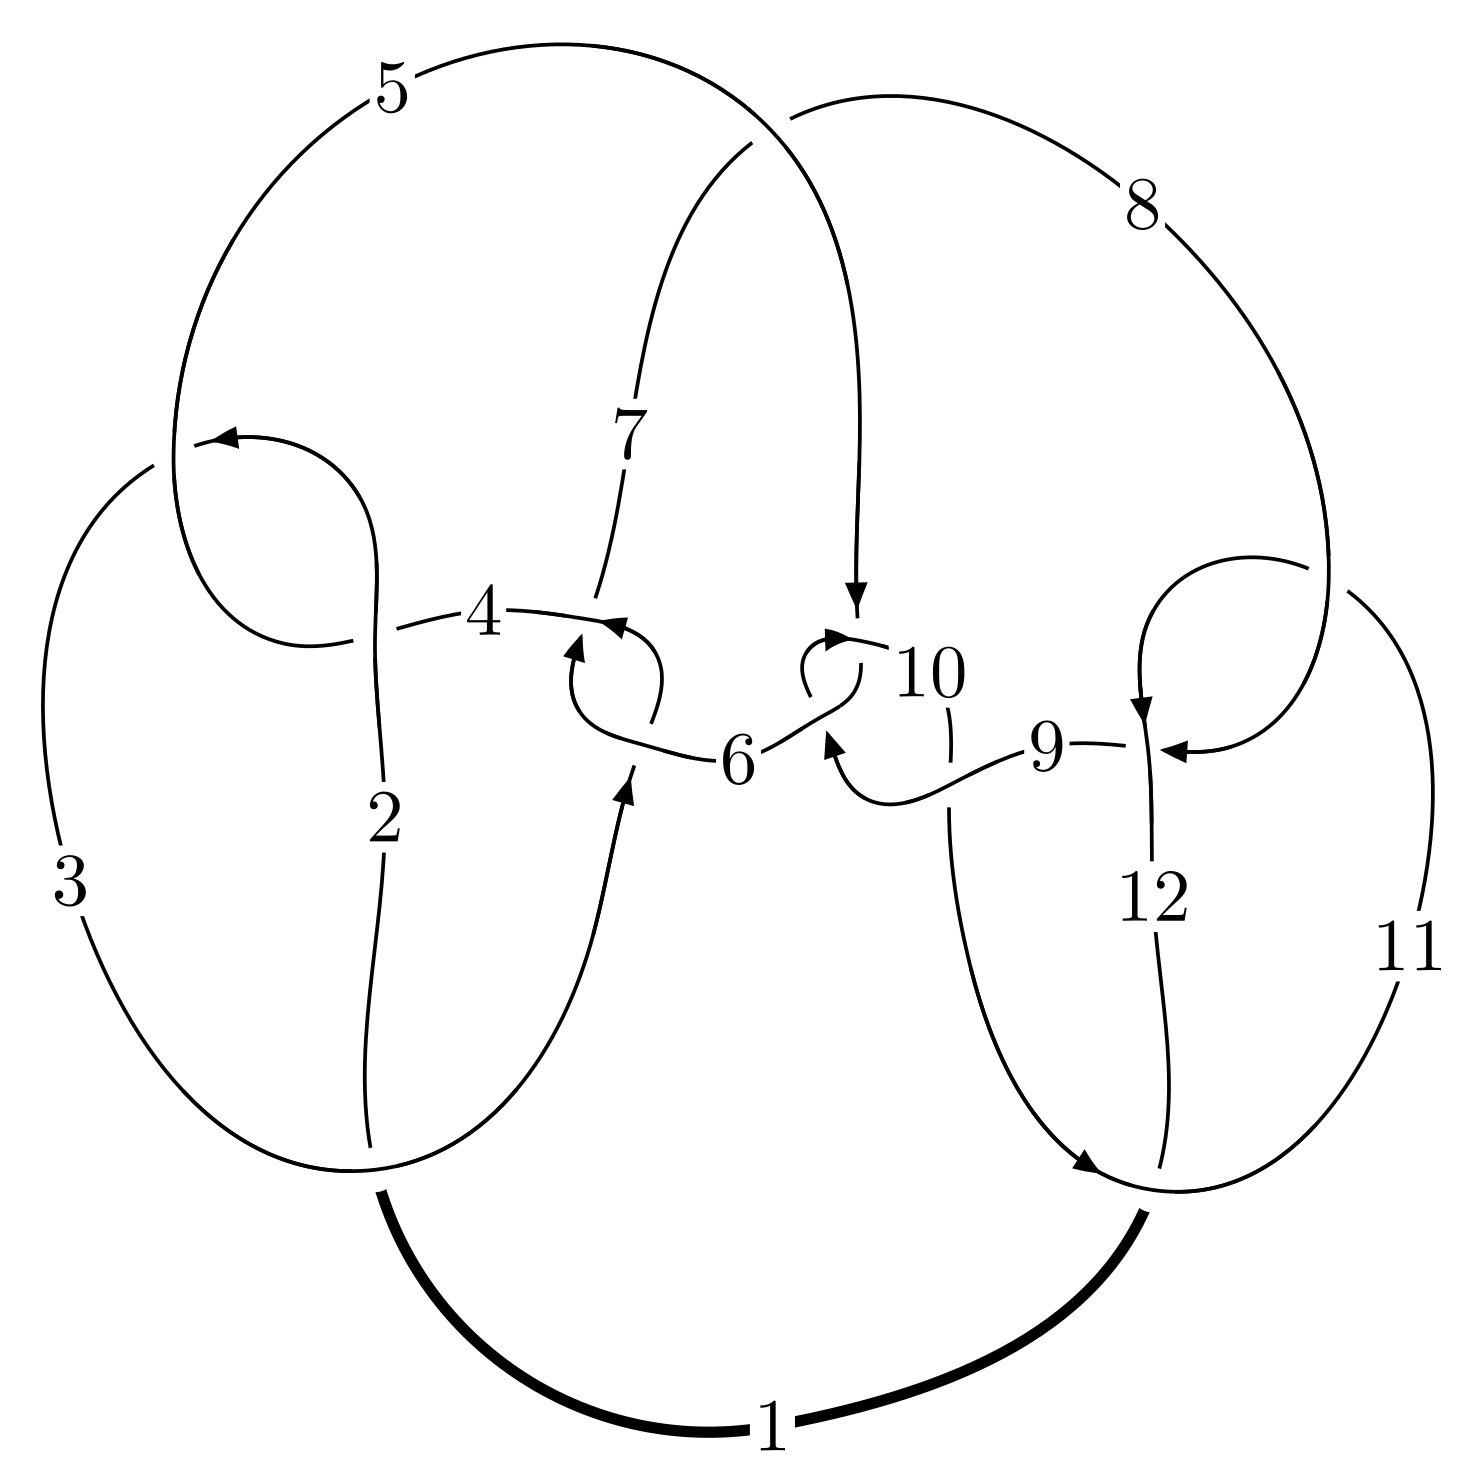
\includegraphics[width=112pt]{../../../GIT/diagram.site/Diagrams/png/2162_12n_0073.png}\\
\ \ \ A knot diagram\footnotemark}&
\allowdisplaybreaks
\textbf{Linearized knot diagam} \\
\cline{2-2}
 &
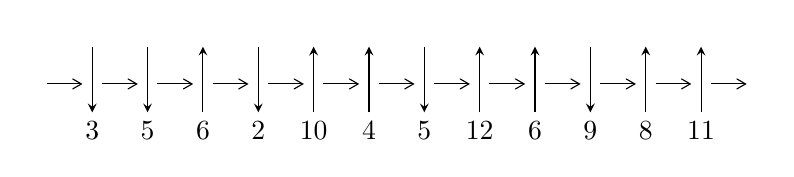
\begin{tikzpicture}[x=20pt, y=17pt]
	% nodes
	\node (C0) at (0, 0) {};
	\node (C1) at (1, 0) {};
	\node (C1U) at (1, +1) {};
	\node (C1D) at (1, -1) {3};

	\node (C2) at (2, 0) {};
	\node (C2U) at (2, +1) {};
	\node (C2D) at (2, -1) {5};

	\node (C3) at (3, 0) {};
	\node (C3U) at (3, +1) {};
	\node (C3D) at (3, -1) {6};

	\node (C4) at (4, 0) {};
	\node (C4U) at (4, +1) {};
	\node (C4D) at (4, -1) {2};

	\node (C5) at (5, 0) {};
	\node (C5U) at (5, +1) {};
	\node (C5D) at (5, -1) {10};

	\node (C6) at (6, 0) {};
	\node (C6U) at (6, +1) {};
	\node (C6D) at (6, -1) {4};

	\node (C7) at (7, 0) {};
	\node (C7U) at (7, +1) {};
	\node (C7D) at (7, -1) {5};

	\node (C8) at (8, 0) {};
	\node (C8U) at (8, +1) {};
	\node (C8D) at (8, -1) {12};

	\node (C9) at (9, 0) {};
	\node (C9U) at (9, +1) {};
	\node (C9D) at (9, -1) {6};

	\node (C10) at (10, 0) {};
	\node (C10U) at (10, +1) {};
	\node (C10D) at (10, -1) {9};

	\node (C11) at (11, 0) {};
	\node (C11U) at (11, +1) {};
	\node (C11D) at (11, -1) {8};

	\node (C12) at (12, 0) {};
	\node (C12U) at (12, +1) {};
	\node (C12D) at (12, -1) {11};
	\node (C13) at (13, 0) {};

	% arrows
	\draw[->,>={angle 60}]
	(C0) edge (C1) (C1) edge (C2) (C2) edge (C3) (C3) edge (C4) (C4) edge (C5) (C5) edge (C6) (C6) edge (C7) (C7) edge (C8) (C8) edge (C9) (C9) edge (C10) (C10) edge (C11) (C11) edge (C12) (C12) edge (C13) ;	\draw[->,>=stealth]
	(C1U) edge (C1D) (C2U) edge (C2D) (C3D) edge (C3U) (C4U) edge (C4D) (C5D) edge (C5U) (C6D) edge (C6U) (C7U) edge (C7D) (C8D) edge (C8U) (C9D) edge (C9U) (C10U) edge (C10D) (C11D) edge (C11U) (C12D) edge (C12U) ;
	\end{tikzpicture} \\
\hhline{~~} \\& 
\textbf{Solving Sequence} \\ \cline{2-2} 
 &
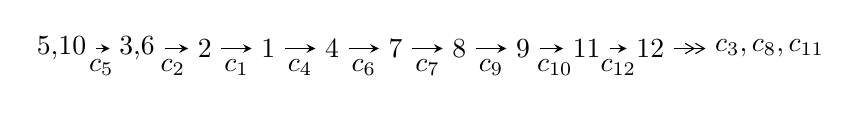
\begin{tikzpicture}[x=23pt, y=7pt]
	% node
	\node (A0) at (-1/8, 0) {5,10};
	\node (A1) at (17/16, 0) {3,6};
	\node (A2) at (17/8, 0) {2};
	\node (A3) at (25/8, 0) {1};
	\node (A4) at (33/8, 0) {4};
	\node (A5) at (41/8, 0) {7};
	\node (A6) at (49/8, 0) {8};
	\node (A7) at (57/8, 0) {9};
	\node (A8) at (65/8, 0) {11};
	\node (A9) at (73/8, 0) {12};
	\node (C1) at (1/2, -1) {$c_{5}$};
	\node (C2) at (13/8, -1) {$c_{2}$};
	\node (C3) at (21/8, -1) {$c_{1}$};
	\node (C4) at (29/8, -1) {$c_{4}$};
	\node (C5) at (37/8, -1) {$c_{6}$};
	\node (C6) at (45/8, -1) {$c_{7}$};
	\node (C7) at (53/8, -1) {$c_{9}$};
	\node (C8) at (61/8, -1) {$c_{10}$};
	\node (C9) at (69/8, -1) {$c_{12}$};
	\node (A10) at (11, 0) {$c_{3},c_{8},c_{11}$};

	% edge
	\draw[->,>=stealth]	
	(A0) edge (A1) (A1) edge (A2) (A2) edge (A3) (A3) edge (A4) (A4) edge (A5) (A5) edge (A6) (A6) edge (A7) (A7) edge (A8) (A8) edge (A9) ;
	\draw[->>,>={angle 60}]	
	(A9) edge (A10);
\end{tikzpicture} \\ 

\end{tabular} \\

\footnotetext{
The image of knot diagram is generated by the software ``\textbf{Draw programme}" developed by Andrew Bartholomew(\url{http://www.layer8.co.uk/maths/draw/index.htm\#Running-draw}), where we modified some parts for our purpose(\url{https://github.com/CATsTAILs/LinksPainter}).
}\phantom \\ \newline 
\centering \textbf{Ideals for irreducible components\footnotemark of $X_{\text{par}}$} 
 
\begin{align*}
I^u_{1}&=\langle 
-3.25963\times10^{16} u^{35}+4.95553\times10^{16} u^{34}+\cdots+3.15381\times10^{17} b+2.76334\times10^{17},\\
\phantom{I^u_{1}}&\phantom{= \langle  }-2.34713\times10^{17} u^{35}+2.08730\times10^{17} u^{34}+\cdots+3.15381\times10^{17} a-4.82090\times10^{17},\;u^{36}-2 u^{35}+\cdots+u-1\rangle \\
I^u_{2}&=\langle 
b+1,\;- u^8+2 u^7-3 u^6+3 u^5-4 u^4+4 u^3-3 u^2+a+2 u-1,\;u^9- u^8+2 u^7- u^6+3 u^5- u^4+2 u^3+u+1\rangle \\
\\
\end{align*}
\raggedright * 2 irreducible components of $\dim_{\mathbb{C}}=0$, with total 45 representations.\\
\footnotetext{All coefficients of polynomials are rational numbers. But the coefficients are sometimes approximated in decimal forms when there is not enough margin.}
\newpage
\renewcommand{\arraystretch}{1}
\centering \section*{I. $I^u_{1}= \langle -3.26\times10^{16} u^{35}+4.96\times10^{16} u^{34}+\cdots+3.15\times10^{17} b+2.76\times10^{17},\;-2.35\times10^{17} u^{35}+2.09\times10^{17} u^{34}+\cdots+3.15\times10^{17} a-4.82\times10^{17},\;u^{36}-2 u^{35}+\cdots+u-1 \rangle$}
\flushleft \textbf{(i) Arc colorings}\\
\begin{tabular}{m{7pt} m{180pt} m{7pt} m{180pt} }
\flushright $a_{5}=$&$\begin{pmatrix}1\\0\end{pmatrix}$ \\
\flushright $a_{10}=$&$\begin{pmatrix}0\\u\end{pmatrix}$ \\
\flushright $a_{3}=$&$\begin{pmatrix}0.744221 u^{35}-0.661834 u^{34}+\cdots-3.44897 u+1.52860\\0.103355 u^{35}-0.157128 u^{34}+\cdots+0.0286142 u-0.876190\end{pmatrix}$ \\
\flushright $a_{6}=$&$\begin{pmatrix}1\\- u^2\end{pmatrix}$ \\
\flushright $a_{2}=$&$\begin{pmatrix}0.847576 u^{35}-0.818962 u^{34}+\cdots-3.42035 u+0.652406\\0.103355 u^{35}-0.157128 u^{34}+\cdots+0.0286142 u-0.876190\end{pmatrix}$ \\
\flushright $a_{1}=$&$\begin{pmatrix}0.376173 u^{35}-0.492061 u^{34}+\cdots+0.281199 u-0.411800\\0.0410701 u^{35}-0.0783542 u^{34}+\cdots-0.108796 u-0.0990764\end{pmatrix}$ \\
\flushright $a_{4}=$&$\begin{pmatrix}0.700268 u^{35}-0.600854 u^{34}+\cdots-3.50274 u+1.47901\\0.106016 u^{35}-0.0966188 u^{34}+\cdots+0.0456405 u-0.849264\end{pmatrix}$ \\
\flushright $a_{7}=$&$\begin{pmatrix}0.376173 u^{35}-0.492061 u^{34}+\cdots+0.281199 u-0.411800\\-0.170748 u^{35}+0.219929 u^{34}+\cdots-0.00709182 u-0.161209\end{pmatrix}$ \\
\flushright $a_{8}=$&$\begin{pmatrix}0.546921 u^{35}-0.711990 u^{34}+\cdots+0.288291 u-0.250591\\-0.170748 u^{35}+0.219929 u^{34}+\cdots-0.00709182 u-0.161209\end{pmatrix}$ \\
\flushright $a_{9}=$&$\begin{pmatrix}- u\\u^3+u\end{pmatrix}$ \\
\flushright $a_{11}=$&$\begin{pmatrix}- u^3\\u^5+u^3+u\end{pmatrix}$ \\
\flushright $a_{12}=$&$\begin{pmatrix}0.267209 u^{35}-0.299525 u^{34}+\cdots+0.309131 u-0.445002\\0.211046 u^{35}-0.287825 u^{34}+\cdots+0.274209 u+0.206608\end{pmatrix}$\\&\end{tabular}
\flushleft \textbf{(ii) Obstruction class $= -1$}\\~\\
\flushleft \textbf{(iii) Cusp Shapes $= \frac{110199305673793977}{315381009766300841} u^{35}+\frac{250535878173710291}{315381009766300841} u^{34}+\cdots-\frac{683728502499797155}{28671000887845531} u+\frac{3186236650537876488}{315381009766300841}$}\\~\\
\newpage\renewcommand{\arraystretch}{1}
\flushleft \textbf{(iv) u-Polynomials at the component}\newline \\
\begin{tabular}{m{50pt}|m{274pt}}
Crossings & \hspace{64pt}u-Polynomials at each crossing \\
\hline $$\begin{aligned}c_{1}\end{aligned}$$&$\begin{aligned}
&u^{36}+2 u^{35}+\cdots+151 u+1
\end{aligned}$\\
\hline $$\begin{aligned}c_{2},c_{4}\end{aligned}$$&$\begin{aligned}
&u^{36}-10 u^{35}+\cdots+19 u-1
\end{aligned}$\\
\hline $$\begin{aligned}c_{3},c_{6}\end{aligned}$$&$\begin{aligned}
&u^{36}+3 u^{35}+\cdots+512 u+512
\end{aligned}$\\
\hline $$\begin{aligned}c_{5},c_{9}\end{aligned}$$&$\begin{aligned}
&u^{36}-2 u^{35}+\cdots+u-1
\end{aligned}$\\
\hline $$\begin{aligned}c_{7}\end{aligned}$$&$\begin{aligned}
&u^{36}-6 u^{35}+\cdots+790797 u-444601
\end{aligned}$\\
\hline $$\begin{aligned}c_{8},c_{11}\end{aligned}$$&$\begin{aligned}
&u^{36}+2 u^{35}+\cdots+5 u+1
\end{aligned}$\\
\hline $$\begin{aligned}c_{10}\end{aligned}$$&$\begin{aligned}
&u^{36}+6 u^{35}+\cdots+u+1
\end{aligned}$\\
\hline $$\begin{aligned}c_{12}\end{aligned}$$&$\begin{aligned}
&u^{36}-22 u^{35}+\cdots+u+1
\end{aligned}$\\
\hline
\end{tabular}\\~\\
\newpage\renewcommand{\arraystretch}{1}
\flushleft \textbf{(v) Riley Polynomials at the component}\newline \\
\begin{tabular}{m{50pt}|m{274pt}}
Crossings & \hspace{64pt}Riley Polynomials at each crossing \\
\hline $$\begin{aligned}c_{1}\end{aligned}$$&$\begin{aligned}
&y^{36}+74 y^{35}+\cdots-20743 y+1
\end{aligned}$\\
\hline $$\begin{aligned}c_{2},c_{4}\end{aligned}$$&$\begin{aligned}
&y^{36}-2 y^{35}+\cdots-151 y+1
\end{aligned}$\\
\hline $$\begin{aligned}c_{3},c_{6}\end{aligned}$$&$\begin{aligned}
&y^{36}-57 y^{35}+\cdots-8126464 y+262144
\end{aligned}$\\
\hline $$\begin{aligned}c_{5},c_{9}\end{aligned}$$&$\begin{aligned}
&y^{36}+6 y^{35}+\cdots+y+1
\end{aligned}$\\
\hline $$\begin{aligned}c_{7}\end{aligned}$$&$\begin{aligned}
&y^{36}+134 y^{35}+\cdots-15572451598723 y+197670049201
\end{aligned}$\\
\hline $$\begin{aligned}c_{8},c_{11}\end{aligned}$$&$\begin{aligned}
&y^{36}-22 y^{35}+\cdots+y+1
\end{aligned}$\\
\hline $$\begin{aligned}c_{10}\end{aligned}$$&$\begin{aligned}
&y^{36}+50 y^{35}+\cdots-35 y+1
\end{aligned}$\\
\hline $$\begin{aligned}c_{12}\end{aligned}$$&$\begin{aligned}
&y^{36}-14 y^{35}+\cdots+61 y+1
\end{aligned}$\\
\hline
\end{tabular}\\~\\
\newpage\flushleft \textbf{(vi) Complex Volumes and Cusp Shapes}
$$\begin{array}{c|c|c}  
\text{Solutions to }I^u_{1}& \I (\text{vol} + \sqrt{-1}CS) & \text{Cusp shape}\\
 \hline 
\begin{aligned}
u &= -0.615843 + 0.841646 I \\
a &= \phantom{-}1.43664 - 0.80379 I \\
b &= \phantom{-}0.301969 + 0.746984 I\end{aligned}
 & \phantom{-}4.77425 - 0.10637 I & \phantom{-}7.48146 + 1.59247 I \\ \hline\begin{aligned}
u &= -0.615843 - 0.841646 I \\
a &= \phantom{-}1.43664 + 0.80379 I \\
b &= \phantom{-}0.301969 - 0.746984 I\end{aligned}
 & \phantom{-}4.77425 + 0.10637 I & \phantom{-}7.48146 - 1.59247 I \\ \hline\begin{aligned}
u &= -0.732748 + 0.745235 I \\
a &= -0.092665 + 1.018320 I \\
b &= \phantom{-}0.079470 - 1.108210 I\end{aligned}
 & \phantom{-}5.18897 - 4.94800 I & \phantom{-}7.17998 + 5.99105 I \\ \hline\begin{aligned}
u &= -0.732748 - 0.745235 I \\
a &= -0.092665 - 1.018320 I \\
b &= \phantom{-}0.079470 + 1.108210 I\end{aligned}
 & \phantom{-}5.18897 + 4.94800 I & \phantom{-}7.17998 - 5.99105 I \\ \hline\begin{aligned}
u &= \phantom{-}0.739358 + 0.601439 I \\
a &= \phantom{-}0.104781 - 0.811350 I \\
b &= \phantom{-}0.083215 + 0.736081 I\end{aligned}
 & \phantom{-}1.62325 + 1.32416 I & \phantom{-}4.12502 - 2.60316 I \\ \hline\begin{aligned}
u &= \phantom{-}0.739358 - 0.601439 I \\
a &= \phantom{-}0.104781 + 0.811350 I \\
b &= \phantom{-}0.083215 - 0.736081 I\end{aligned}
 & \phantom{-}1.62325 - 1.32416 I & \phantom{-}4.12502 + 2.60316 I \\ \hline\begin{aligned}
u &= \phantom{-}0.125468 + 1.044610 I \\
a &= \phantom{-}0.966320 + 0.109826 I \\
b &= \phantom{-}0.454746 - 0.102565 I\end{aligned}
 & -2.34146 + 2.27465 I & \phantom{-}2.44627 - 4.29475 I \\ \hline\begin{aligned}
u &= \phantom{-}0.125468 - 1.044610 I \\
a &= \phantom{-}0.966320 - 0.109826 I \\
b &= \phantom{-}0.454746 + 0.102565 I\end{aligned}
 & -2.34146 - 2.27465 I & \phantom{-}2.44627 + 4.29475 I \\ \hline\begin{aligned}
u &= -0.912979 + 0.603282 I \\
a &= -0.094847 + 0.581208 I \\
b &= \phantom{-}0.428044 - 0.685537 I\end{aligned}
 & \phantom{-}4.35891 + 2.74036 I & \phantom{-}7.57970 - 3.16606 I \\ \hline\begin{aligned}
u &= -0.912979 - 0.603282 I \\
a &= -0.094847 - 0.581208 I \\
b &= \phantom{-}0.428044 + 0.685537 I\end{aligned}
 & \phantom{-}4.35891 - 2.74036 I & \phantom{-}7.57970 + 3.16606 I\\
 \hline 
 \end{array}$$\newpage$$\begin{array}{c|c|c}  
\text{Solutions to }I^u_{1}& \I (\text{vol} + \sqrt{-1}CS) & \text{Cusp shape}\\
 \hline 
\begin{aligned}
u &= \phantom{-}0.552810 + 1.007290 I \\
a &= \phantom{-}1.032000 + 0.667957 I \\
b &= \phantom{-}0.536480 - 0.548160 I\end{aligned}
 & \phantom{-}0.20181 + 3.58839 I & \phantom{-}2.59766 - 4.47078 I \\ \hline\begin{aligned}
u &= \phantom{-}0.552810 - 1.007290 I \\
a &= \phantom{-}1.032000 - 0.667957 I \\
b &= \phantom{-}0.536480 + 0.548160 I\end{aligned}
 & \phantom{-}0.20181 - 3.58839 I & \phantom{-}2.59766 + 4.47078 I \\ \hline\begin{aligned}
u &= \phantom{-}0.403187 + 0.692172 I \\
a &= \phantom{-}0.222101 - 1.316930 I \\
b &= -0.848909 + 0.718608 I\end{aligned}
 & -0.01273 + 3.75640 I & \phantom{-}1.96178 - 8.67374 I \\ \hline\begin{aligned}
u &= \phantom{-}0.403187 - 0.692172 I \\
a &= \phantom{-}0.222101 + 1.316930 I \\
b &= -0.848909 - 0.718608 I\end{aligned}
 & -0.01273 - 3.75640 I & \phantom{-}1.96178 + 8.67374 I \\ \hline\begin{aligned}
u &= -0.656810 + 1.069490 I \\
a &= \phantom{-}0.849616 - 0.843755 I \\
b &= \phantom{-}0.705777 + 0.623024 I\end{aligned}
 & \phantom{-}2.76036 - 8.54206 I & \phantom{-}5.00446 + 8.46696 I \\ \hline\begin{aligned}
u &= -0.656810 - 1.069490 I \\
a &= \phantom{-}0.849616 + 0.843755 I \\
b &= \phantom{-}0.705777 - 0.623024 I\end{aligned}
 & \phantom{-}2.76036 + 8.54206 I & \phantom{-}5.00446 - 8.46696 I \\ \hline\begin{aligned}
u &= \phantom{-}0.959801 + 0.917573 I \\
a &= -0.795562 - 0.722155 I \\
b &= \phantom{-}1.04335 + 1.28065 I\end{aligned}
 & \phantom{-}15.4107 + 4.2831 I & \phantom{-}6.51475 - 3.16359 I \\ \hline\begin{aligned}
u &= \phantom{-}0.959801 - 0.917573 I \\
a &= -0.795562 + 0.722155 I \\
b &= \phantom{-}1.04335 - 1.28065 I\end{aligned}
 & \phantom{-}15.4107 - 4.2831 I & \phantom{-}6.51475 + 3.16359 I \\ \hline\begin{aligned}
u &= -0.110883 + 0.661998 I \\
a &= -0.567675 + 0.716209 I \\
b &= -1.295050 - 0.200690 I\end{aligned}
 & -2.17080 - 1.28901 I & -2.65057 + 3.66135 I \\ \hline\begin{aligned}
u &= -0.110883 - 0.661998 I \\
a &= -0.567675 - 0.716209 I \\
b &= -1.295050 + 0.200690 I\end{aligned}
 & -2.17080 + 1.28901 I & -2.65057 - 3.66135 I\\
 \hline 
 \end{array}$$\newpage$$\begin{array}{c|c|c}  
\text{Solutions to }I^u_{1}& \I (\text{vol} + \sqrt{-1}CS) & \text{Cusp shape}\\
 \hline 
\begin{aligned}
u &= -0.981174 + 0.904102 I \\
a &= -0.759912 + 0.643457 I \\
b &= \phantom{-}1.05191 - 1.17838 I\end{aligned}
 & \phantom{-}11.26030 + 0.66616 I & \phantom{-}3.25844 + 0.20862 I \\ \hline\begin{aligned}
u &= -0.981174 - 0.904102 I \\
a &= -0.759912 - 0.643457 I \\
b &= \phantom{-}1.05191 + 1.17838 I\end{aligned}
 & \phantom{-}11.26030 - 0.66616 I & \phantom{-}3.25844 - 0.20862 I \\ \hline\begin{aligned}
u &= \phantom{-}0.914043 + 0.991327 I \\
a &= \phantom{-}0.58196 + 1.72130 I \\
b &= \phantom{-}1.10681 - 1.16652 I\end{aligned}
 & \phantom{-}15.1611 + 2.6010 I & \phantom{-}6.17050 - 1.49093 I \\ \hline\begin{aligned}
u &= \phantom{-}0.914043 - 0.991327 I \\
a &= \phantom{-}0.58196 - 1.72130 I \\
b &= \phantom{-}1.10681 + 1.16652 I\end{aligned}
 & \phantom{-}15.1611 - 2.6010 I & \phantom{-}6.17050 + 1.49093 I \\ \hline\begin{aligned}
u &= \phantom{-}1.000680 + 0.916853 I \\
a &= -0.805879 - 0.579891 I \\
b &= \phantom{-}1.13554 + 1.14001 I\end{aligned}
 & \phantom{-}15.0538 - 5.8256 I & \phantom{-}6.10110 + 2.81591 I \\ \hline\begin{aligned}
u &= \phantom{-}1.000680 - 0.916853 I \\
a &= -0.805879 + 0.579891 I \\
b &= \phantom{-}1.13554 - 1.14001 I\end{aligned}
 & \phantom{-}15.0538 + 5.8256 I & \phantom{-}6.10110 - 2.81591 I \\ \hline\begin{aligned}
u &= -0.914948 + 1.013510 I \\
a &= \phantom{-}0.49309 - 1.64704 I \\
b &= \phantom{-}1.15250 + 1.09178 I\end{aligned}
 & \phantom{-}10.89350 - 7.61965 I & \phantom{-}2.72159 + 4.20211 I \\ \hline\begin{aligned}
u &= -0.914948 - 1.013510 I \\
a &= \phantom{-}0.49309 + 1.64704 I \\
b &= \phantom{-}1.15250 - 1.09178 I\end{aligned}
 & \phantom{-}10.89350 + 7.61965 I & \phantom{-}2.72159 - 4.20211 I \\ \hline\begin{aligned}
u &= \phantom{-}0.931682 + 1.021610 I \\
a &= \phantom{-}0.39982 + 1.67662 I \\
b &= \phantom{-}1.22688 - 1.08995 I\end{aligned}
 & \phantom{-}14.6962 + 12.8981 I & \phantom{-}5.54056 - 6.97685 I \\ \hline\begin{aligned}
u &= \phantom{-}0.931682 - 1.021610 I \\
a &= \phantom{-}0.39982 - 1.67662 I \\
b &= \phantom{-}1.22688 + 1.08995 I\end{aligned}
 & \phantom{-}14.6962 - 12.8981 I & \phantom{-}5.54056 + 6.97685 I\\
 \hline 
 \end{array}$$\newpage$$\begin{array}{c|c|c}  
\text{Solutions to }I^u_{1}& \I (\text{vol} + \sqrt{-1}CS) & \text{Cusp shape}\\
 \hline 
\begin{aligned}
u &= \phantom{-}0.473309 + 0.394862 I \\
a &= \phantom{-}2.44876 - 1.56604 I \\
b &= -0.697476 - 0.163056 I\end{aligned}
 & \phantom{-}0.829785 - 0.751885 I & \phantom{-}3.89282 - 2.36905 I \\ \hline\begin{aligned}
u &= \phantom{-}0.473309 - 0.394862 I \\
a &= \phantom{-}2.44876 + 1.56604 I \\
b &= -0.697476 + 0.163056 I\end{aligned}
 & \phantom{-}0.829785 + 0.751885 I & \phantom{-}3.89282 + 2.36905 I \\ \hline\begin{aligned}
u &= -0.261492 + 0.555195 I \\
a &= -0.24853 + 1.82453 I \\
b &= -0.984945 - 0.277413 I\end{aligned}
 & -1.87419 - 0.91390 I & -3.92701 + 0.44517 I \\ \hline\begin{aligned}
u &= -0.261492 - 0.555195 I \\
a &= -0.24853 - 1.82453 I \\
b &= -0.984945 + 0.277413 I\end{aligned}
 & -1.87419 + 0.91390 I & -3.92701 - 0.44517 I \\ \hline\begin{aligned}
u &= \phantom{-}0.560238\phantom{ +0.000000I} \\
a &= \phantom{-}0.651078\phantom{ +0.000000I} \\
b &= \phantom{-}0.0833533\phantom{ +0.000000I}\end{aligned}
 & \phantom{-}1.12215\phantom{ +0.000000I} & \phantom{-}9.27350\phantom{ +0.000000I} \\ \hline\begin{aligned}
u &= -0.387160\phantom{ +0.000000I} \\
a &= \phantom{-}9.00889\phantom{ +0.000000I} \\
b &= -1.04399\phantom{ +0.000000I}\end{aligned}
 & -0.292584\phantom{ +0.000000I} & \phantom{-}54.7300\phantom{ +0.000000I}\\
 \hline 
 \end{array}$$\newpage\newpage\renewcommand{\arraystretch}{1}
\centering \section*{II. $I^u_{2}= \langle b+1,\;- u^8+2 u^7+\cdots+a-1,\;u^9- u^8+2 u^7- u^6+3 u^5- u^4+2 u^3+u+1 \rangle$}
\flushleft \textbf{(i) Arc colorings}\\
\begin{tabular}{m{7pt} m{180pt} m{7pt} m{180pt} }
\flushright $a_{5}=$&$\begin{pmatrix}1\\0\end{pmatrix}$ \\
\flushright $a_{10}=$&$\begin{pmatrix}0\\u\end{pmatrix}$ \\
\flushright $a_{3}=$&$\begin{pmatrix}u^8-2 u^7+3 u^6-3 u^5+4 u^4-4 u^3+3 u^2-2 u+1\\-1\end{pmatrix}$ \\
\flushright $a_{6}=$&$\begin{pmatrix}1\\- u^2\end{pmatrix}$ \\
\flushright $a_{2}=$&$\begin{pmatrix}u^8-2 u^7+3 u^6-3 u^5+4 u^4-4 u^3+3 u^2-2 u\\-1\end{pmatrix}$ \\
\flushright $a_{1}=$&$\begin{pmatrix}-1\\0\end{pmatrix}$ \\
\flushright $a_{4}=$&$\begin{pmatrix}u^8-2 u^7+3 u^6-3 u^5+4 u^4-4 u^3+3 u^2-2 u+1\\-1\end{pmatrix}$ \\
\flushright $a_{7}=$&$\begin{pmatrix}1\\- u^2\end{pmatrix}$ \\
\flushright $a_{8}=$&$\begin{pmatrix}u^2+1\\- u^2\end{pmatrix}$ \\
\flushright $a_{9}=$&$\begin{pmatrix}- u\\u^3+u\end{pmatrix}$ \\
\flushright $a_{11}=$&$\begin{pmatrix}- u^3\\u^5+u^3+u\end{pmatrix}$ \\
\flushright $a_{12}=$&$\begin{pmatrix}u^8+u^6+u^4-1\\- u^8+u^7- u^6+2 u^5- u^4+2 u^3+2 u+1\end{pmatrix}$\\&\end{tabular}
\flushleft \textbf{(ii) Obstruction class $= 1$}\\~\\
\flushleft \textbf{(iii) Cusp Shapes $= -3 u^8-4 u^6+3 u^5-10 u^4+u^3-7 u^2+6 u-4$}\\~\\
\newpage\renewcommand{\arraystretch}{1}
\flushleft \textbf{(iv) u-Polynomials at the component}\newline \\
\begin{tabular}{m{50pt}|m{274pt}}
Crossings & \hspace{64pt}u-Polynomials at each crossing \\
\hline $$\begin{aligned}c_{1},c_{2}\end{aligned}$$&$\begin{aligned}
&(u-1)^9
\end{aligned}$\\
\hline $$\begin{aligned}c_{3},c_{6}\end{aligned}$$&$\begin{aligned}
&u^9
\end{aligned}$\\
\hline $$\begin{aligned}c_{4}\end{aligned}$$&$\begin{aligned}
&(u+1)^9
\end{aligned}$\\
\hline $$\begin{aligned}c_{5}\end{aligned}$$&$\begin{aligned}
&u^9- u^8+2 u^7- u^6+3 u^5- u^4+2 u^3+u+1
\end{aligned}$\\
\hline $$\begin{aligned}c_{7},c_{10}\end{aligned}$$&$\begin{aligned}
&u^9+3 u^8+8 u^7+13 u^6+17 u^5+17 u^4+12 u^3+6 u^2+u-1
\end{aligned}$\\
\hline $$\begin{aligned}c_{8}\end{aligned}$$&$\begin{aligned}
&u^9- u^8-2 u^7+3 u^6+u^5-3 u^4+2 u^3- u+1
\end{aligned}$\\
\hline $$\begin{aligned}c_{9}\end{aligned}$$&$\begin{aligned}
&u^9+u^8+2 u^7+u^6+3 u^5+u^4+2 u^3+u-1
\end{aligned}$\\
\hline $$\begin{aligned}c_{11}\end{aligned}$$&$\begin{aligned}
&u^9+u^8-2 u^7-3 u^6+u^5+3 u^4+2 u^3- u-1
\end{aligned}$\\
\hline $$\begin{aligned}c_{12}\end{aligned}$$&$\begin{aligned}
&u^9-5 u^8+12 u^7-15 u^6+9 u^5+u^4-4 u^3+2 u^2+u-1
\end{aligned}$\\
\hline
\end{tabular}\\~\\
\newpage\renewcommand{\arraystretch}{1}
\flushleft \textbf{(v) Riley Polynomials at the component}\newline \\
\begin{tabular}{m{50pt}|m{274pt}}
Crossings & \hspace{64pt}Riley Polynomials at each crossing \\
\hline $$\begin{aligned}c_{1},c_{2},c_{4}\end{aligned}$$&$\begin{aligned}
&(y-1)^9
\end{aligned}$\\
\hline $$\begin{aligned}c_{3},c_{6}\end{aligned}$$&$\begin{aligned}
&y^9
\end{aligned}$\\
\hline $$\begin{aligned}c_{5},c_{9}\end{aligned}$$&$\begin{aligned}
&y^9+3 y^8+8 y^7+13 y^6+17 y^5+17 y^4+12 y^3+6 y^2+y-1
\end{aligned}$\\
\hline $$\begin{aligned}c_{7},c_{10}\end{aligned}$$&$\begin{aligned}
&y^9+7 y^8+20 y^7+25 y^6+5 y^5-15 y^4+22 y^2+13 y-1
\end{aligned}$\\
\hline $$\begin{aligned}c_{8},c_{11}\end{aligned}$$&$\begin{aligned}
&y^9-5 y^8+12 y^7-15 y^6+9 y^5+y^4-4 y^3+2 y^2+y-1
\end{aligned}$\\
\hline $$\begin{aligned}c_{12}\end{aligned}$$&$\begin{aligned}
&y^9- y^8+12 y^7-7 y^6+37 y^5+y^4-10 y^2+5 y-1
\end{aligned}$\\
\hline
\end{tabular}\\~\\
\newpage\flushleft \textbf{(vi) Complex Volumes and Cusp Shapes}
$$\begin{array}{c|c|c}  
\text{Solutions to }I^u_{2}& \I (\text{vol} + \sqrt{-1}CS) & \text{Cusp shape}\\
 \hline 
\begin{aligned}
u &= -0.140343 + 0.966856 I \\
a &= -1.004430 + 0.297869 I \\
b &= -1.00000\phantom{ +0.000000I}\end{aligned}
 & -3.42837 - 2.09337 I & -6.19892 + 4.26451 I \\ \hline\begin{aligned}
u &= -0.140343 - 0.966856 I \\
a &= -1.004430 - 0.297869 I \\
b &= -1.00000\phantom{ +0.000000I}\end{aligned}
 & -3.42837 + 2.09337 I & -6.19892 - 4.26451 I \\ \hline\begin{aligned}
u &= -0.628449 + 0.875112 I \\
a &= -0.275254 + 0.816341 I \\
b &= -1.00000\phantom{ +0.000000I}\end{aligned}
 & -1.02799 - 2.45442 I & -0.00914 + 2.54651 I \\ \hline\begin{aligned}
u &= -0.628449 - 0.875112 I \\
a &= -0.275254 - 0.816341 I \\
b &= -1.00000\phantom{ +0.000000I}\end{aligned}
 & -1.02799 + 2.45442 I & -0.00914 - 2.54651 I \\ \hline\begin{aligned}
u &= \phantom{-}0.796005 + 0.733148 I \\
a &= \phantom{-}0.070080 - 0.850995 I \\
b &= -1.00000\phantom{ +0.000000I}\end{aligned}
 & \phantom{-}2.72642 - 1.33617 I & \phantom{-}5.35644 + 0.59665 I \\ \hline\begin{aligned}
u &= \phantom{-}0.796005 - 0.733148 I \\
a &= \phantom{-}0.070080 + 0.850995 I \\
b &= -1.00000\phantom{ +0.000000I}\end{aligned}
 & \phantom{-}2.72642 + 1.33617 I & \phantom{-}5.35644 - 0.59665 I \\ \hline\begin{aligned}
u &= \phantom{-}0.728966 + 0.986295 I \\
a &= -0.195086 - 0.635552 I \\
b &= -1.00000\phantom{ +0.000000I}\end{aligned}
 & \phantom{-}1.95319 + 7.08493 I & \phantom{-}3.81555 - 4.89194 I \\ \hline\begin{aligned}
u &= \phantom{-}0.728966 - 0.986295 I \\
a &= -0.195086 + 0.635552 I \\
b &= -1.00000\phantom{ +0.000000I}\end{aligned}
 & \phantom{-}1.95319 - 7.08493 I & \phantom{-}3.81555 + 4.89194 I \\ \hline\begin{aligned}
u &= -0.512358\phantom{ +0.000000I} \\
a &= \phantom{-}3.80937\phantom{ +0.000000I} \\
b &= -1.00000\phantom{ +0.000000I}\end{aligned}
 & -0.446489\phantom{ +0.000000I} & -9.92790\phantom{ +0.000000I}\\
 \hline 
 \end{array}$$\newpage
\newpage\renewcommand{\arraystretch}{1}
\centering \section*{ III. u-Polynomials}
\begin{tabular}{m{50pt}|m{274pt}}
Crossings & \hspace{64pt}u-Polynomials at each crossing \\
\hline $$\begin{aligned}c_{1}\end{aligned}$$&$\begin{aligned}
&((u-1)^9)(u^{36}+2 u^{35}+\cdots+151 u+1)
\end{aligned}$\\
\hline $$\begin{aligned}c_{2}\end{aligned}$$&$\begin{aligned}
&((u-1)^9)(u^{36}-10 u^{35}+\cdots+19 u-1)
\end{aligned}$\\
\hline $$\begin{aligned}c_{3},c_{6}\end{aligned}$$&$\begin{aligned}
&u^9(u^{36}+3 u^{35}+\cdots+512 u+512)
\end{aligned}$\\
\hline $$\begin{aligned}c_{4}\end{aligned}$$&$\begin{aligned}
&((u+1)^9)(u^{36}-10 u^{35}+\cdots+19 u-1)
\end{aligned}$\\
\hline $$\begin{aligned}c_{5}\end{aligned}$$&$\begin{aligned}
&(u^9- u^8+\cdots+u+1)(u^{36}-2 u^{35}+\cdots+u-1)
\end{aligned}$\\
\hline $$\begin{aligned}c_{7}\end{aligned}$$&$\begin{aligned}
&(u^9+3 u^8+8 u^7+13 u^6+17 u^5+17 u^4+12 u^3+6 u^2+u-1)\\
&\cdot(u^{36}-6 u^{35}+\cdots+790797 u-444601)
\end{aligned}$\\
\hline $$\begin{aligned}c_{8}\end{aligned}$$&$\begin{aligned}
&(u^9- u^8+\cdots- u+1)(u^{36}+2 u^{35}+\cdots+5 u+1)
\end{aligned}$\\
\hline $$\begin{aligned}c_{9}\end{aligned}$$&$\begin{aligned}
&(u^9+u^8+\cdots+u-1)(u^{36}-2 u^{35}+\cdots+u-1)
\end{aligned}$\\
\hline $$\begin{aligned}c_{10}\end{aligned}$$&$\begin{aligned}
&(u^9+3 u^8+8 u^7+13 u^6+17 u^5+17 u^4+12 u^3+6 u^2+u-1)\\
&\cdot(u^{36}+6 u^{35}+\cdots+u+1)
\end{aligned}$\\
\hline $$\begin{aligned}c_{11}\end{aligned}$$&$\begin{aligned}
&(u^9+u^8+\cdots- u-1)(u^{36}+2 u^{35}+\cdots+5 u+1)
\end{aligned}$\\
\hline $$\begin{aligned}c_{12}\end{aligned}$$&$\begin{aligned}
&(u^9-5 u^8+12 u^7-15 u^6+9 u^5+u^4-4 u^3+2 u^2+u-1)\\
&\cdot(u^{36}-22 u^{35}+\cdots+u+1)
\end{aligned}$\\
\hline
\end{tabular}\newpage\renewcommand{\arraystretch}{1}
\centering \section*{ IV. Riley Polynomials}
\begin{tabular}{m{50pt}|m{274pt}}
Crossings & \hspace{64pt}Riley Polynomials at each crossing \\
\hline $$\begin{aligned}c_{1}\end{aligned}$$&$\begin{aligned}
&((y-1)^9)(y^{36}+74 y^{35}+\cdots-20743 y+1)
\end{aligned}$\\
\hline $$\begin{aligned}c_{2},c_{4}\end{aligned}$$&$\begin{aligned}
&((y-1)^9)(y^{36}-2 y^{35}+\cdots-151 y+1)
\end{aligned}$\\
\hline $$\begin{aligned}c_{3},c_{6}\end{aligned}$$&$\begin{aligned}
&y^9(y^{36}-57 y^{35}+\cdots-8126464 y+262144)
\end{aligned}$\\
\hline $$\begin{aligned}c_{5},c_{9}\end{aligned}$$&$\begin{aligned}
&(y^9+3 y^8+8 y^7+13 y^6+17 y^5+17 y^4+12 y^3+6 y^2+y-1)\\
&\cdot(y^{36}+6 y^{35}+\cdots+y+1)
\end{aligned}$\\
\hline $$\begin{aligned}c_{7}\end{aligned}$$&$\begin{aligned}
&(y^9+7 y^8+20 y^7+25 y^6+5 y^5-15 y^4+22 y^2+13 y-1)\\
&\cdot(y^{36}+134 y^{35}+\cdots-15572451598723 y+197670049201)
\end{aligned}$\\
\hline $$\begin{aligned}c_{8},c_{11}\end{aligned}$$&$\begin{aligned}
&(y^9-5 y^8+12 y^7-15 y^6+9 y^5+y^4-4 y^3+2 y^2+y-1)\\
&\cdot(y^{36}-22 y^{35}+\cdots+y+1)
\end{aligned}$\\
\hline $$\begin{aligned}c_{10}\end{aligned}$$&$\begin{aligned}
&(y^9+7 y^8+20 y^7+25 y^6+5 y^5-15 y^4+22 y^2+13 y-1)\\
&\cdot(y^{36}+50 y^{35}+\cdots-35 y+1)
\end{aligned}$\\
\hline $$\begin{aligned}c_{12}\end{aligned}$$&$\begin{aligned}
&(y^9- y^8+12 y^7-7 y^6+37 y^5+y^4-10 y^2+5 y-1)\\
&\cdot(y^{36}-14 y^{35}+\cdots+61 y+1)
\end{aligned}$\\
\hline
\end{tabular}
\vskip 2pc
\end{document}